\documentclass[12pt,twoside]{report} 
\usepackage[utf8]{inputenc}

\usepackage{geometry}
\geometry{a4paper}
\usepackage{url}
\usepackage{graphicx} 
\usepackage{booktabs} 
\usepackage{array} 
\usepackage{paralist} 
\usepackage{verbatim} 
\usepackage{subfig} 
\usepackage{amsmath}
\usepackage{fancyhdr} 
\pagestyle{fancy} 
\renewcommand{\headrulewidth}{0pt} 
\lhead{}\chead{}\rhead{}
\lfoot{}\cfoot{\thepage}\rfoot{}
\usepackage{fullpage}
\usepackage[active]{srcltx}

\usepackage{sectsty}
\allsectionsfont{\sffamily\mdseries\upshape}


\usepackage[nottoc,notlof,notlot]{tocbibind} 
\usepackage[titles,subfigure]{tocloft} 
\renewcommand{\cftsecfont}{\rmfamily\mdseries\upshape}
\renewcommand{\cftsecpagefont}{\rmfamily\mdseries\upshape} 



\title{Bioremediation}
\author{Ivan Marin}
\date{\today} 

\begin{document}
\maketitle
\tableofcontents




%=================================================================================================
\chapter{Bioremediation}
\section{Biological Degradation}

\section{First order degradation}
The biodegradation of organic contaminants can be modeled using a first order differential equation for the concentration of the substrate (organic contaminant) in function of time:
\begin{align}\label{firstorder}
\frac{dC}{dt} = -aC
\end{align}
The solution of equation \eqref{firstorder} is equal to
\begin{align}
C = C_{0}e^{-kt}
\end{align}
where 
\begin{itemize}
\item C: present concentration of the substrate
\item $C_{0}$: starting concentration
\item k: decrease rate of the substrate [$T^{-1}$]
\end{itemize}
This model assumes that solute degradation rate is proportional to the solute concentration. It's a simple model that can represent some systems, needing only one parameter to be determined. It does not include effects like availability of electron acceptors or electron donors. This representation is also not capable of include effects as adaptation, inhibition, preferential substrate utilization and growth of the microorganism population \cite{schirmer_relative-least-squares_1999}.


\section{Monod Kinetics}
Other model largely used to model biodegradation is the Monod or Michaelis-Menten kinetics \cite{monod, appelo}. This model can consider substrate and biomass levels and its interaction. The Monod equations can also be extended to include the effects of limitation of electron acceptors. This model with electron acceptors is usually called dual Monod equations. The concentration of the microorganisms can be included as a static concentration or can be modeled also using a Monod equation.

The Monod model is described by the Monod kinetic rate equation: 
\begin{align}
\frac{dC}{dt} = - k_{max} M \frac{C}{k_{\frac{1}{2}} + C}
\end{align}
where
\begin{itemize}
\item C: present concentration of the substrate
\item $k_{max}$: maximum rate consumption of the substrate, [$mg/L/s$] or [$\text{kg substrate/kg bacteria/d}$]
\item $k_{\frac{1}{2}}$: half-utilization rate, the concentration where the degradation is occuring at half the maximum rate [$kg/m^{3}$]
\item M: concentration of the microorganisms [$kg/m^3$]
\end{itemize}
It should be noted that some authors include the microorganism mass in the $k_max$ constant, differently when $\mu_{max}$ is used.  



The limiting cases for the Monod equation are: when the concentration $C$ is smaller than the half utilization rate, $C << k_{\frac{1}{2}}$ and when the opposite is true, $C >> k_{\frac{1}{2}}$. In the first case the Monod equation is reduced to a first order equation:
\begin{align}
\frac{dC}{dt} = - \frac{k_{max} M} {k_{\frac{1}{2}}}C
\end{align}
The second case $C >> k_{\frac{1}{2}}$ leads to a zero order rate equation:
\begin{align}
\frac{dC}{dt} = -k_{max} M
\end{align}

\subsection{Dual Monod equations}
To include the effects of the limitation of the electron acceptors in the biodegradation process a second term is used in the Monod equation:

\begin{align}
\frac{dC}{dt} = - k_{max} M \frac{C}{k_{\frac{1}{2}} + C}\frac{A}{k_{A\frac{1}{2}} + A}\left( \frac{1}{R}\right)
\end{align}
where 
\begin{itemize}
\item A: concentration of the electron acceptor [$kg/m^{3}/d$]
\item $k_{A\frac{1}{2}}$: half-utilization rate for the electron acceptor [$kg/m^3$]
\end{itemize}

A differential equation must be also written for the electron acceptor:

\begin{align}
\frac{dA}{dt} = - k_{max} X M \frac{C}{k_{\frac{1}{2}} + C}\frac{A}{k_{A\frac{1}{2}} + A} \left( \frac{1}{R}\right)
\end{align}
 where 
\begin{itemize}
\item X: stochiometric ratio between the utilization of the substrate and the consumption of the electron acceptor, [kg EA/kg S]
\end{itemize}

\subsubsection{Microorganism mass growth and chemical description}
The growth of the microorganism population can be modeled by a similar dual Monod equation: 

\begin{align}
\frac{dM}{dt} = - k_{max} Y M \frac{C}{k_{\frac{1}{2}} + C}\frac{A}{k_{A\frac{1}{2}} + A} - bM
\end{align}
where
\begin{itemize}
\item M: concentration of the microorganisms, [$kg/m^{3}$]
\item Y: yield factor, the fraction of the substrate that is converted to biomass [kg microorganism / kg substrate] or [mol C microorganism / mol C in substrate]
\item b: linear decay rate for the microorganisms, [$day^{-1}$]
\end{itemize}

There are attempts to describe chemically the microorganisms in the literature, but no consensus. Usually is not important for simulations, but when the equations are written in $mol/L$ units, a $g/mol$ relation must be established. \cite{appelo} uses the formula $CH_{1.4}O_{0.4}N_{0.2}$, with $22.6 g/mol$. 

\subsection{Units transformations}
The microbiology literature usually presents the experimental data in $mg/L$ and days. To transform back and forth to BIONAPL and Phreeqc some conversions are necessary. Assuming that the bacteria mass is equal to $22,6 g/mol$, $k_max$, given in $[kg substrate / kg bacteria/day]$ must be transformed to $[mol substrate/ mol bacteria/s]$ using the conversion

\begin{align}
k_{max} * \frac{\text{molecular mass substrate}}{\text{molecular mass bacteria} \times 86400 }
\end{align}

For example, the conversion from $4,13 \text{kg substrate}/\text{kg bacteria}\times d^{-1}$ is 
\begin{align}
4,13 \times \frac{1/106.16e-3}{1/22.6e-3} \times \frac{1}{86400} = 1.017e-5 \frac{\text{mol substrate}}{\text{mol bacteria}\times s}
\end{align} 

The fractions are equivalent as 1 kg substrate = 1 / molecular weight substrate and the same for the bacteria.

For the yield $Y$ the same rule applies. When using $mol/L$ concentrations, the factor should be adjusted to $\text{mol bacteria / mol C in the substrate}$. For example, in the degradation of xylene ($C8H10$) with molecular weight of $106,16 g/mol$, the yield given in $mg/mg$ in \cite{schirmer} of $0,52$ must be converted as $0,52 \times \frac{1/22,6}{1/106,16}$ what is equal to $2,44 \text{mol biomass}/\text{mol xylene}$. 

\subsection{Relationship between Michaelis-Menten approach and Monod equations}
The Monod equation includes the constant $k_{max}$ that relates to the substrate. This parameter can be described also in function of the growth rate of the microorganisms:

\begin{align}
k_{max} = \frac{\mu_{max}}{Y}M
\end{align}
where
\begin{itemize}
\item $\mu_{max}$: maximum microorganism growth rate, [$day^{-1}$]
\end{itemize}
Care should be taken when reviewing the literature, as some authors list $k_{max}$ and others $\mu_{max}$.

\subsection{Haldane Inhibition}
As \cite{schirmer_relative-least-squares_1999} points out, some higher concentrations of the substrate can be toxic for the microoorganisms, delaying the biodegradation. This effect can be represented by the Haldane Inhibition, given by 
\begin{align}
\frac{dC}{dt} = - k_{max} M \frac{C}{k_{\frac{1}{2}} + C + \frac{C^2}{K_{I}}}\frac{A}{k_{A\frac{1}{2}} + A}
\end{align}
where
\begin{itemize}
\item $K_{I}$: Haldane inhibition constant [$kg/m^3$]
\end{itemize}


\chapter{Comparison of Phreeqc and BIONAPL}
\section{Comparison of Phreeqc and BIONAPL results with experimental data for biodegradation with excess of oxygen}
A script for Phreeqc was written to simulate the biodegradation of m-xylene in a batch microcosm reaction in excess of oxygen, and teh results were compared with the experimental data from \cite{schirmer_relative-least-squares_1999} batch microcosm experiment. The parameters used were derived from \cite{schirmer_relative-least-squares_1999} and are listed in table \eqref{tableparam}:

\begin{center}
    \begin{tabular}{ | l | c | c |}
    \hline
              & BIONAPL ($kg$, $m$, $d$) & Phreeqc ($mol$, $l$, $s$ ) \\ 
    \hline
    $k_{max}$ &         4,13 d-1         &    1,017e-5 mol xyl/mol bac s-1           \\ 
    \hline
    $k_{\frac{1}{2}}$ & 0,00079 kg/m3    &   7,441e-6 mol/l           \\ 
    \hline
    $k_{I}$           &      ---         &   8,65e-4 mol/l            \\
    \hline
    Y                 &     0,52         &    2,44 mol bac/mol xyl    \\
    \hline
    Init. microorg.   &    3e-6 kg/m3    &    1,33e-7 mol/l           \\
    \hline
    Init. Xylene      &     0,0047 kg/m3 -0,037.3 kg/m3 &     4,7mg/l - 37,3 mg/l                 \\
    \hline
    Retardation       &       2e-4        &   0,86                     \\
    \hline
    \end{tabular}\label{tableparam}
\end{center}

The graphs \eqref{1}-\eqref{4} show the comparison of both BIONAPL and Phreeqc without the term for electron acceptor in the Monod equations. The agreement of both simulations is high when the concentration is low and there is no Haldane inhibition in Phreeqc. The scenario changes when the initial concentration of xylene is higher: xylene can be toxic when in higher concentrations. Both simulations agree when the concetration is higher, but not with the data points from \cite{schirmer_relative-least-squares_1999}. When Haldane inhibition is included in Phreeqc it agrees with the data points. 
\begin{figure}[h]
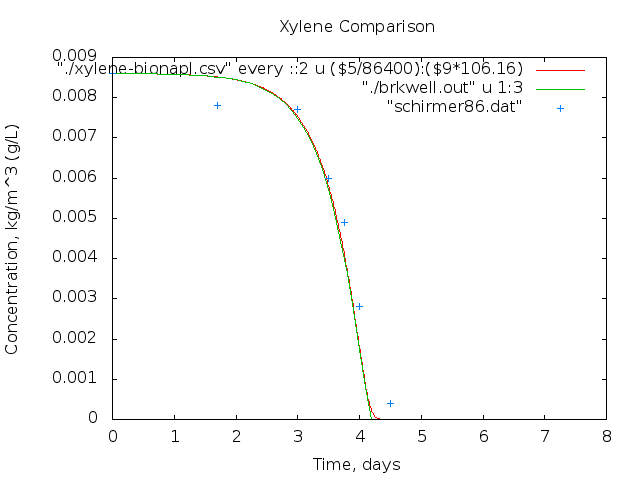
\includegraphics[width=12cm]{img/comp-xylene86nohaldane.png}
\caption{Comparison of BIONAPL and Phreeqc without Haldane inhibition activated in the Phreeqc simulation. Initial xylene concentration: 8,6 mg/l.}
\label{1}
\end{figure}

\begin{figure}[h]
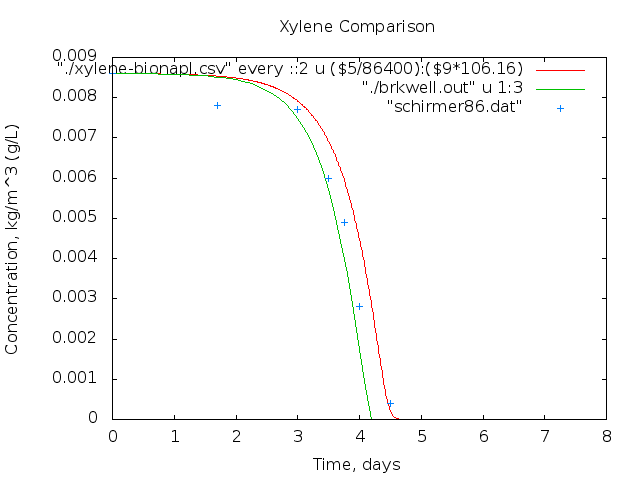
\includegraphics[width=14cm]{img/comp-xylene86haldane.png}
\caption{Comparison of BIONAPL and Phreeqc with Haldane inhibition activated in the Phreeqc simulation. Initial xylene concentration: 8,6 mg/l.}
\label{2}
\end{figure}

\begin{figure}[h]
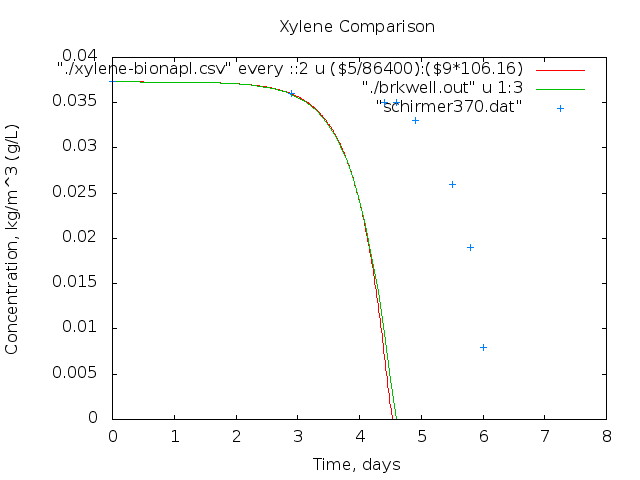
\includegraphics[width=14cm]{img/comp-xylene37nohaldane.png}
\caption{Comparison of BIONAPL and Phreeqc without Haldane inhibition activated in the Phreeqc simulation. Initial xylene concentration: 37,3 mg/l.}
\label{3}
\end{figure}


\begin{figure}[h]
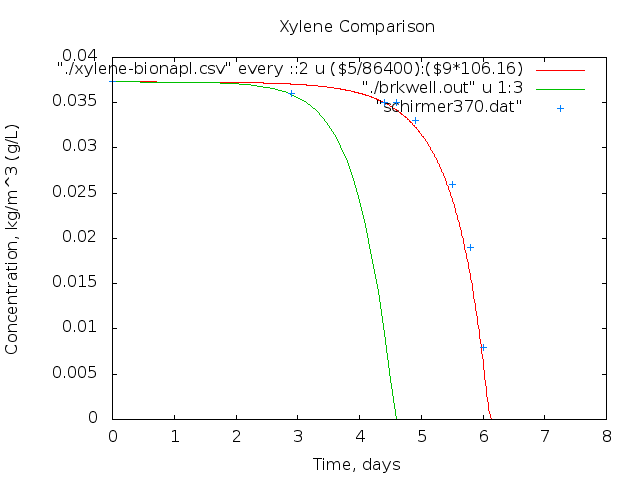
\includegraphics[width=14cm]{img/comp-xylene37haldane.png}
\caption{Comparison of BIONAPL and Phreeqc with Haldane inhibition activated in the Phreeqc simulation. Initial xylene concentration: 37,3 mg/l.}
\label{4}
\end{figure}


\begin{figure}[h]
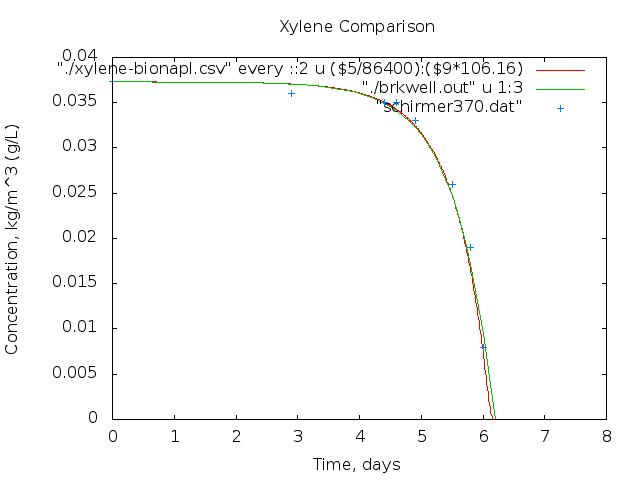
\includegraphics[width=14cm]{img/comp-xylene37fullhaldane.png}
\caption{Comparison of BIONAPL and Phreeqc with Haldane inhibition activated in both simulations. Initial xylene concentration: 37,3 mg/l.}
\label{4}
\end{figure}


\chapter{Scripts and Input Files used}
\section{Phreeqc}
\begin{verbatim}
TITLE CompBIONAPL 2
# This model degrades xylene using a Monod
# equation and biomass generation. The results
# will be compared with a similar simulation using
# BIONAPL.

SOLUTION_MASTER_SPECIES
  Xylene   Xylene       0     C8H10  106.16

SOLUTION_SPECIES
  Xylene = Xylene
  log_k 0
  -gamma    0.0000    0.0000

RATES
 Xylene_degradation
 -start
  1 K_max = parm(1)
  2 K_half = parm(2)
  3 KI = parm(3)  
  4 R = 1 + parm(4)
  5 Y = parm(5)
 10 S = mol("Xylene")
 20 if S < 1e-15 then goto 60
 30 B = kin("Biomass")
 40 rate =  - K_max * B * (S /(K_half + S + (S*S/KI))) / R
 #40 rate =  -  K_max * (B/Y) * (S / (K_half + S )) / R
 50 dS = rate * time
 60 save dS
 70 put(rate, 1)
 -end

 Biomass
 -start
  1 Y = parm(1)
  2 R = 1 + parm(2)
  3 k_Bd = parm(3)
 10 rate = get(1) * R
 20 B = kin("Biomass")
 30 rate = - Y * rate - k_Bd * B
 40 dB = rate * time
 50 save -dB
 60 print kin("Biomass")
 -end


 KINETICS 1
 Xylene_degradation
  -formula Xylene 1 
  -m0 0
  -parms 1.017e-5  7.45e-6  8.65e-4  0.86  2.44 # K_max (s-1), K_half(mol/L), KI(mol/L), R, Y
  
 Biomass
   -formula C 0
   -m0 1.33e-7
   -parms  2.44  0.86  0         # Y, R, K_Bd

  -steps 6.3e5 in 700

INCREMENTAL_REACTIONS

SOLUTION 1
 -units mg/l
 Xylene 37.3

 SELECTED_OUTPUT
   -file xylene-bionapl.csv
   -molalities Xylene 
   -kinetic_reactants Biomass
END
\end{verbatim}
\section{BIONAPL input file}
\begin{verbatim}
BIONAPL MODEL + +   1D, single-EA  2D 
106x8x30 elements  - 
January 2013
 0  2  0  0  0  0  0  0  0  1 1 0 1 ;kp,kcn,kwt,kint,kintv,kgo,kg,kranb,krans,kbio,mode,keqm;krtype
   1    1    1               ngx, ngy, ngz  # of uniform sections per direction
   1.           ;xlim    length of section
   1.                     ;ylim    in [m]
   1.                        ;zlim     Aquifer thickness
   1                  ;nlx    # of elements per section
   1                       ;nly
   1                         ;nlz
 00   00.   0.0    0.0   1500.        ;nwtl,datum,gamma,sdecay,rhob
    1   1   1   1   -1       ;ix,iy,iz1,iz2 breakthrough recorded at wells
    0                                    ;INIT
    1   1   1   2   1   1   10.00  -1 ; initial condition head
    0   0   0   0   0   0      2     1     0.0000      -1    ;fractures
     0   0   0   0   0    0            ;B.C.'S (FLOW) fixed flow at upper B
    1  1     1.e-4  1.e-4   1.e-4  0.35        -1   ;1-NEL,KX,KY,KZ (m/s),porosity
    1  1  1  1  1   1  1.e-4   1.e-4   1.e-4 0.35 -1   ;inner source   K of source,por
  1   1  1   1   1     -1                 ;fence definition
  0.0e-3  0.01   1.5e-4              ;SS,srw,gradius
  1   1           xlam   b    Kc       Km     DD       ;# of components,# of EA
Xylene 
870.  .106  .198   1.0  0.0  2.00e-4   0.     5.6e-10  0 0. 0.0917  ;rho,mw,aqs,Sh,b,kc,km,D,kdp,xdp,khaldane
  1   2  1  2  1  2     -1           ;Source distribution on xyz//
  0.0               ;moles
  4.13  0.00079   1e-20  0.00   0.52   99999.  ;utils (/day),uhs,uho,ros,ym,cinib Toluene + O2
  0.                                                           ;inhibition 
  1.  .000001       ;RETO1,kinib1
  1000.    0.00e-10     .1          ;retm,bm,ymmax
   0.5  3.0e-6             ;BACKGROUND CONC. O1,O2..-M1.M2   (obsolete)
   0.5  3.0e-6             ;INITIAL SOURCE CONC. O-M         (obsolete)
 0.000001   0.000001 0.000001  0.000001                ;threshold S,O1,O2...
   1  2   1  2   1  2   1  37.3e-3    37.3e-3    +1  ;initial condition
   1  2   1  2   1  2   3  0.005   0.005    -1  ;initial condition O2 
 0   0   0   0   0    0           ;B.C.'S (ORGANIC TRANSPORT) - L R, N F, B T
 0   0   0   0   0    0           ;B.C.'S (HA TRANSPORT) - L R, N F, B T
 0   0   0   0   0   0           ;B.C.'S (O2 TRANSPORT) - L R, N F, B T
    0.0e-4    1.  0. 1. 0.                    ;ka,n,xmtc,feqm,qha(kgHA/kgsol)
    1       1.0e-10       0.       0.   ;IVEL,VX,VY,VZ (m/s) v=q/n(=K*i/por)
 1 1 1  1  1 1  1.0 .02  .01   0.000   -1    ;AL,ATH,ATV,decay(bckgnd)by elm
.0001  0.0001 2  20                          ;CCP,CCW,MAXIT1,MAXIT2
  1.0    1.00                              ;OVER-RELAX HEADS,temp
   1    0    0   0   0               ;KNOX(1)(2)TRANSV. SECTION
   0    0    0    0    0                  ;KNOY(1),(2)LONG.  SECTION
   1                                      ;knoz
 1825.  3650. 7300. 10950.   36500.          ;five 3d print times (days)
  0.   7.  0.1   99999  99999 99999 -1             ;t0,t1,dt,kplot(afterXtimesteps),kmom,kflow
 1.                                           ;new % ccc
  0.000    1.     0.0    0                  ;hinc,rinc,eqmfact(kg),kha(transport of hum.acid)
  1.0                                       ;massfact (multiplyer)
  1.0   1.0                                    ;sfact (ncomp+1)
    1  1  1  1  1  0.00e-5  0.0  0.10  -1         ;i,j,k1,k2,kcc,pqq,tqq,radius,more







 730. 10950.  10.  73 9999  -1             ;t0,t1,dt,kplot(afterXtimesteps),kmom
 1.                                            ;new % ccc
  0.000    1.     0.0    0                  ;hinc,rinc,eqmfact,kha(transport of hum.acid)
  1.0                                       ;massfact
  1.0   1.0                                    ;sfact (ncomp+1)
    36 1  18  18  1  0.00e-5  0.0  0.10  -1         ;i,j,k1,k2,kcc,pqq,tqq,radius,more

 10950. 36500.  10.  73 9999  +1           ;t0,t1,dt,kplot(afterXtimesteps),kmom
 1.                                            ;new % ccc
  0.000    1.     0.0    0                  ;hinc,rinc,eqmfact,kha(transport of hum.acid)
  1.0                                       ;massfact
  1.0   1.0                                    ;sfact (ncomp+1)
    36 1  18  18  1  0.00e-5  0.0  0.10  -1         ;i,j,k1,k2,kcc,pqq,tqq,radius,more
 36500.  109500.  10.  73 9999  -1         ;t0,t1,dt,kplot(afterXtimesteps),kmom
 1.                                            ;new % ccc
  0.000    1.     0.0    0                  ;hinc,rinc,eqmfact,kha(transport of hum.acid)
  1.0                                       ;massfact
  1.0   1.0                                    ;sfact (ncomp+1)
    36 1  18  18  1  0.00e-5  0.0  0.10  -1         ;i,j,k1,k2,kcc,pqq,tqq,radius,more



 109500.  146000.  10.  73 9999  -1         ;t0,t1,dt,kplot(afterXtimesteps),kmom
 1.                                            ;new % ccc
  0.000    1.     0.0    0                  ;hinc,rinc,eqmfact,kha(transport of hum.acid)
  1.0                                       ;massfact
  1.0   1.0                                    ;sfact (ncomp+1)
    36 1  18  18  1  0.00e-5  0.0  0.10  -1         ;i,j,k1,k2,kcc,pqq,tqq,radius,more

\end{verbatim}



\bibliographystyle{plain}
\bibliography{bibliografia/bibliografia}
\end{document}